\documentclass[a4paper]{article}
\usepackage[UTF8]{ctex}
\usepackage{geometry}
\usepackage{graphicx}
\usepackage{url}
\usepackage{multirow}
\usepackage{array}
\usepackage{booktabs}
\usepackage{url}
\usepackage{enumitem}
\usepackage{graphicx}
\usepackage{float}
\usepackage{amssymb}
\usepackage{amsmath}
\usepackage{subfig}
\usepackage{longtable}
\usepackage{pifont}
\usepackage{color}

\allowdisplaybreaks

\geometry{a4paper, scale=0.78}

% \begin{figure}[H]
%     \centering
%     \includegraphics[width=.55\textwidth]{E.png}
%     \caption{矩阵与列向量的乘法}
%     \label{fig:my_label_1}
% \end{figure}

% \left\{
% \begin{array}{ll}
%       x+2x+z=2 & \\
%       3x+8y+z=12 & \\
%       4y+z=2
% \end{array}
% \right.

% \begin{enumerate}[itemindent = 1em, itemsep = 0.4pt, parsep=0.5pt, topsep = 0.5pt]

% \end{enumerate}

%\stackrel{a}{\longrightarrow}

\title{Probability Graph 08 Belief Propagation}
\author{Chen Gong}
\date{08 December 2019}
\begin{document}
\maketitle

在上一小节中,我们已经介绍了变量消除(Variable Elimination),Variable Elimination的思想是Probability Graph中的核心思想之一。上一节中我们就已经介绍了,这实际上就是乘法对加法的分配律。但是,Variable Elimination中有很多的问题,比如重复计算和最优计算次序不好确定的问题。所以,我们这一节来介绍Belief Propagation来解决重复计算的问题。

\section{Forward and Backward Algorithm}
假设,我们现在有一个马氏链模型:
\begin{figure}[H]
    \centering
    
\includegraphics[width=.45\textwidth]{微信图片_20191208140942.png}
    \caption{链式马氏链模型结构图}
    \label{fig:my_label_1}
\end{figure}

联合概率可以被我们表示为:$p(a,b,c,d,e)=p(a)\cdot p(b|a)\cdot p(c|b)\cdot p(d|c) \cdot p(e|d)$。

如果,我们想要求的是$p(e)$,那么:
\begin{equation}
    \begin{split}
            p(e) 
            = & \sum_{a,b,c,d}p(a,b,c,d,e) \\
            = & \sum_{a}p(e|d)\cdot\sum_cp(d|c)\cdot\sum_bp(c|b)\cdot\sum_ap(b|a)\cdot p(a)
    \end{split}
\end{equation}

为了简化表达,这里我们需要定义一个很重要的符号。因为,$\sum_ap(b|a)\cdot p(a)$,是一个关于$b$的表达式,也就是相当于把$a$给约掉了。所以我们可以把$\sum_ap(b|a)\cdot p(a)$记为$m_{a\longrightarrow b}(b)$。同理,我们也可以将$\sum_cp(d|c)\cdot\sum_bp(c|b)\cdot m_{a\longrightarrow b}(b)$记为$m_{b\longrightarrow c}(c)$。那么为了求得$p(e)$,我们依次的求解顺序为$m_{a\longrightarrow b}(b)$,$m_{b\longrightarrow c}(c)$,$m_{c\longrightarrow d}(d)$和$m_{d\longrightarrow e}(e)$。也就相当于沿着这个链这个马氏链一直往前走,也就是前向算法(Forward Algorithm)。我们用公式表达即为:
\begin{equation}
    a \stackrel{m_{a\longrightarrow b}(b)}{\longrightarrow} b \stackrel{m_{b\longrightarrow c}(c)}{\longrightarrow} c \stackrel{m_{c\longrightarrow d}(d)}{\longrightarrow} d \stackrel{m_{d\longrightarrow e}(e)}{\longrightarrow} e 
\end{equation}

如果是要求$p(c)$,那么我们的传递过程为$a\longrightarrow b \longrightarrow c \longleftarrow d \longleftarrow e$。这里,我们就不能只用前向算法来解决了,需要用到Forward-Backward算法来解决了。也就是同时使用Forward和Backward的方法,那么我们来看看$p(c)$怎么求?
\begin{equation}
    \begin{split}
        p(c) 
        = & \sum_{a,b,d,e}p(a,b,c,d,e) \\
        = & (\sum_b p(c|b)\sum_a p(b|a)p(a)) \cdot (\sum_d p(d|c)\sum_e p(e|d)) \\
    \end{split}
\end{equation}

对比上面的计算$p(e)$的过程,我们就可以发现,$\sum_b p(c|b)\sum_a p(b|a)p(a)$部分的计算也就是$m_{b\longrightarrow c}(c)$的计算是一模一样的。所以说,Variable Elimination里面有大量的重复计算。Belief的想法很简单,也就是将$m_{i\longrightarrow j}(j)$,全部事先计算好,就像一个个积木一样,然后再用这个积木来搭建运算。那么也就是,我们事先将方向全部定义好,正向和反向的全部都求了再说。为了进一步探究Belief Background,我们需要讨论一些更加Generalize的情况。也就是从Chain$\longrightarrow$Tree,有向$\longrightarrow$无项的情况。

\section{Belief Propagation的扩展}
我们的Generalize的后,分析了一个树形的无向图结构。图的网络结构如下所示:
\begin{figure}[H]
    \centering
    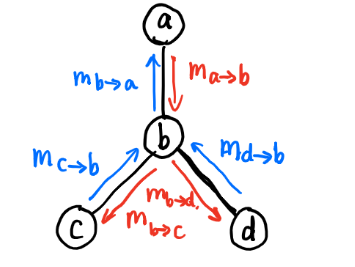
\includegraphics[width=.35\textwidth]{微信图片_20191208145754.png}
    \caption{树形无向图结构拓扑结构}
    \label{fig:my_label_1}
\end{figure}

下面第一步,我们把上面那个模型的设置写出来。所以,我们需要进行因式分解,我们用$\varphi(i)$来表示和$i$有关的部分。所以,我们可以将联合概率密度写为:
\begin{equation}
    p(a,b,c,d) = \frac{1}{Z} \varphi_a(a)\varphi_b(b)\varphi_c(c)\varphi_d(d)\cdot \varphi_{a,b}(a,b)\varphi_{b,c}(b,c)\varphi_{b,d}(b,d)
\end{equation}

我们要求$p(a) = \sum_{b,c,d}p(a,b,c,d)$和$p(b) = \sum_{a,c,d}p(a,b,c,d)$,其间一定会出现大量的重复计算。这个模型中有四个点,三条边,每条边都有两个方向,所以我们要求的是6个“积木”。我们来一步步的看看,如何可以得到想要的$p(a)$。

1. 首先,我们需要求的是$c\longrightarrow b$和$d \longrightarrow b$两个过程。其中,$c\longrightarrow b$的过程也就是$m_{c\longrightarrow b}(b)$,可以被我们表达为$\sum_c \varphi_c\cdot \varphi_{b,c}$。同理,$m_{d\longrightarrow b}(b)$可以被我们表达为$\sum_d \varphi_b\cdot \varphi_{b,d}$。

2. 第二步,我们需要求$b\longrightarrow a$的过程,也就是$m_{b\longrightarrow a}(a)$。它等于$m_{c\longrightarrow b}(b),m_{d\longrightarrow b}(b)$乘上$b$自己的部分求和得到,我们可以写为:
\begin{equation}
    m_{b\longrightarrow a}(a) = \sum_b m_{c\longrightarrow b}(b)\cdot \varphi_b\cdot\varphi_{a,b}\cdot m_{d\longrightarrow b}(b)
\end{equation}

3. 最后,$m_{b\longrightarrow a}(a)$乘上$a$自己的部分就得到了$p(a)$,也就是:$p(a) = \varphi_a \cdot m_{b\longrightarrow a}(a)$。

所以,我们总结一下:
\begin{equation}
    m_{b\longrightarrow a}(x_a) = \sum_{x_b} \varphi_{a,b}\varphi_bm_{c\longrightarrow b}(x_b)m_{d\longrightarrow b}(x_b)
\end{equation}

而,
\begin{equation}
    p(a) = \varphi_a m_{b \longrightarrow a}(x_a)
\end{equation}

我相信到这里,大家应该是可以理解这个意思的,会有点抽象,但并不是很难。下一步我想做个Generalize为了便于大家进行理解,我这里尽量不跳步:
\begin{equation}
    m_{b\longrightarrow a}(x_a) = \sum_{x_b} \varphi_{a,b}\varphi_b \prod_{\{k \in NB(b)\}\longrightarrow a } m_{k\longrightarrow b}(x_b)
\end{equation}

这里的$NB(b)$代表的是所有节点$b$的邻接节点。我们可以进一步表示为:
\begin{equation}
    m_{j\longrightarrow i}(x_i) = \sum_{x_j} \varphi_{i,j}\varphi_j \prod_{\{k \in NB(j)\}\longrightarrow i } m_{k\longrightarrow j}(x_j)
\end{equation}

而,
\begin{equation}
    p(x_i) = \varphi_i \prod_{k\in NB(i)} m_{k\Longrightarrow i}(x_i)
\end{equation}

通过对上面表达式的观察,我们是不是发现了一个很有意思的现象。也就是这些概率都是由$m_{i\longrightarrow j}$这样的小积木拼接起来的。所以我们可以get a conclusion:{\color{red} 我们不要一上来就直接去求边缘概率密度,比如$p(a),p(b),p(c),p(d)$这些的。我们可以先建立一个Cache,把$m_{i\longrightarrow j}$全部算出来。然后,要求什么的话,直接进行搭建和拼接就可以了。}从这里,我们就引出了Belief Propagation。

\section{Belief Propagation}
我们之前就已经得到了信息传递的表达式:
\begin{equation}
    m_{b\longrightarrow a}=\sum_{b}\varphi_{a,b}\varphi_b \cdot m_{c\longrightarrow b}\cdot m_{d\longrightarrow b}
\end{equation}

在开始理解Belief Propagation之前,我们在分析一下$m_{b\longrightarrow a}$的公式中,每个部分表达的具体含义。其中,$m_{c\longrightarrow b}\cdot m_{d\longrightarrow b}$中反映的是孩子(Children)的信息。而$\varphi_b$中表示是$b$节点自己的信息。那么,$\varphi_b \cdot m_{c\longrightarrow b}\cdot m_{d\longrightarrow b}$可以被我们看成是$b$节点的所有信息,包括节点自己本身的信息和其他节点传播来的信息,所以我们将这个部分记为:Belief。所以,Belief$(b)=\varphi_b\cdot$ children。$b$节点收集孩子和自己的信息,整合和$b$相关的所有信息,通过Belief$(b)=\varphi_b\cdot$ children向$a$传去。

那么,Belief Propagation可以看成是BP = VE + Cashing。这个算法的核心思想就在于,直接求$m_{i\longrightarrow j}$,然后再导出边缘概率$p(x_i)$。第二小节中我们已经详细的给出了$p(x_i)$的推导方法。下一步,我们需要知道如何来求$m_{i\longrightarrow j}$。

\subsection{Sequential Implementation}
顺序计算的思路,我们需要借助一个队列来实现:

1. Get Root: 首先我们需要假设一个节点为根节点。

2. Collect Message: 对于每一个在根节点的邻接点中的节点$x_i$,Collect Message ($x_i$)。对应的就是图2中蓝色的线条。

3. Distribute Message: 对于每一个在根节点的邻接点中的节点$x_i$,Distribute Message ($x_i$)。对应的就是图2中红色的线条。

经过这三个步骤以后,我们可以得到所有的$i,j\in v$,从而计算出$p(x_k),k\in v$。

\subsection{Parallel Implementation}
这种思想在图结构的网络中经常使用,大致也就是随意选一个节点,然后向四周其他的节点辐射信息。其他节点收到信息之后,更新自己的状态,然后反馈自己的信息给源节点,源节点再更新自己的信息。不断地重复这个工作,直到最后收敛为止。

\section{小结}
实际上,Belief Propagation就是一种Variable Elimination。但是,我们发现了Variable Elimination中有很多的重复计算。所以,我们想到了提取出来先算好,要用的时候直接放进去就行了。所以,Belief Propagation中分解了传递的过程,先计算消息传递的机制,再来组装出计算边缘概率。其实本质还是Variable Elimination算法,不过就是使表达更加的规范了,通过拆解的方法来消除重复计算。

\end{document}
